%%%%%%%%%%%%%%%%%%%%%%%%%%%%%%%%%%%%%%%%%%%%%%%%%%
%%%%%%%%%%%%%%%%%%%%%%%%%%%%%%%%%%%%%%%%%%%%%%%%%%
%%
%% Based one the "beamer-greek-two" template provided 
%% by the Laboratory of Computational Mathematics, 
%% Mathematical Software and Digital Typography, 
%% Department of Mathematics, University of the Aegean
%% (http://myria.math.aegean.gr/labs/dt/)
%%
%% Adapted by John Liaperdos, October-November 2014
%% (ioannis.liaperdos@gmail.com)
%%
%% Last update: 22/06/2017 (English Support)
%% Source: https://es.overleaf.com/latex/templates/thesis-presentation-template-beamer-english-version-dpt-of-computer-engineering-technological-educational-institute-of-peloponnese/vwhtyshhtqmg
%%%%%%%%%%%%%%%%%%%%%%%%%%%%%%%%%%%%%%%%%%%%%%%%%%
%%%%%%%%%%%%%%%%%%%%%%%%%%%%%%%%%%%%%%%%%%%%%%%%%%
%%
\PassOptionsToPackage{unicode}{hyperref}
\PassOptionsToPackage{naturalnames}{hyperref}
\documentclass{beamer} 
\usepackage{babel}
\usepackage[utf8]{inputenc}
\usepackage{multicol}
\usepackage{caption}
\usepackage{subfig}

%%% FONT SELECTION %%%%%%%%%%%%%%%%%
%%% we choose a sans font %%%%%%%%%%
\usepackage{kmath,kerkis} 
%\usepackage[default]{gfsneohellenic} 
%%%%%%%%%%%%%%%%%%%%%%%%%%%%%%%%%%%%

\usepackage{color}
\usepackage{amsmath}
\usepackage{amssymb}

\usepackage{epstopdf}
\usepackage{graphicx}
\graphicspath{{./img/}}

%%
% load TEI-Pel - specific layout
\usepackage{TeiPel_En_Beamer_Layout}
\setTeipelLayout{draft,newlogo}% options: "draft", "newlogo"

%%%%%%%%%%%%%%%%%%%%%%%%%%%%%%%%%%%%%%%%%%%%%%%%%%%%%%%%%%%%
% Thesis Info %%%%%%%%%%%%%%%%%%%%%%%%%%%%%%%%%%%%%%%%%%%%%%
%%%%%%%%%%%%%%%%%%%%%%%%%%%%%%%%%%%%%%%%%%%%%%%%%%%%%%%%%%%%
	% title
		\title[Análisis de redes causales en deportes de equipo]{Análisis de redes causales en deportes de equipo}	
	% author 
    % (In the mandatory argument "{}", separate multiple
    % authors with "\and" - use "\\" for better author name formatting
    % in the title page. In the optional argument "[]" include all
	% author names, with no "\and" or text formatting macros.)
	% Example: 
    %\author[A. Author Albert Einstein]{Anthony Author \and Albert Einstein}
		\author[E. Merelo]{Elena Merelo Molina}
	% supervisor	
		% \supervisor{Supervisor}{Mister Supervisor}{Professor}
	% date
		\presentationDate{7 de septiembre de 2022}
%%%%%%%%%%%%%%%%

\begin{document}

% typeset front slides
	\typesetFrontSlides

%%%%%%%%%%%%%%%%
% Your Slides Start here:

%%%%
\section{Introducción}

%%
\subsection[Problema]{Descripción del problema}

\begin{frame}{Motivación}
	\framesubtitle{El fútbol es un deporte de equipo \textit{complejo}}
    Como parte del cuerpo técnico de un equipo habrá que decidir:
    \begin{itemize}
		\item Quién será convocado y quién jugará
        \item Cuándo y qué cambios habrá
        \item Alineación por la que se abogará
        \item A quién fichar o vender, qué hacer en los entrenamientos,... 
	\end{itemize}
\end{frame}

\begin{frame}{Descripción}
	\begin{itemize}
		\item ¿Analizar la entropía sobre el grafo de pases nos ayuda a entender mejor el desempeño de un equipo?
		\item ¿Hasta qué punto es determinante la entropía a nivel de jugador o equipo?
        \item ¿Es posible ver la entropía reflejada en un tipo de visualización de las redes de pases?
	\end{itemize}
\end{frame}

\begin{frame}{Metodología}
	\begin{itemize}
		\item \textbf{Desarrollo ágil}
		\item \textit{Design thinking}
	\end{itemize}
\end{frame}

%%
\subsection{Definiciones}
\begin{frame}{Grafos}
	\begin{definition}
		$\mathcal{G} = (V, E)$, con $V$ conjunto finito de vértices distinguibles y 
		$E \subseteq V \times V$ conjunto de aristas. Un par ordenado $(u, v) \in E$ denota un borde dirigido
		del vértice $u$ al vértice $v$. Los bordes dirigidos se representarán con flechas. 
	\end{definition}
	En nuestro caso, representaremos las redes de pases mediante grafos no dirigidos, donde los nodos serán las 
	jugadoras, y los arcos los pases.
\end{frame}

\begin{frame}{Redes bayesianas}
    \begin{definition}[Redes bayesianas] 
        Una red bayesiana $\mathfrak{B} = \lbrace \mathcal{G}, \mathbb{P} \rbrace$ está definida por:
        \begin{itemize}
            \item $\mathcal{G}=(V,E)$ 
            \item $(\Omega, \mathbb{P})$.
            \item $\textbf{V}=V[i], i=1,...,N$, $(\Omega, \mathbb{P})$ 
            de tal manera que $\mathbb{P}(V[1],...,V[N])= \prod_{i=1}^{n}\mathbb{P}(V[i]|pa(V[i]))$
			% la probabilidad conjunta es el productorio de las probabilidades condicionadas
        \end{itemize}
    \end{definition}  
	El cálculo de la probabilidad conjunta que se usa en la entropía coincide con el modelo 
	probabilístico de la red bayesiana.
\end{frame}

\begin{frame}{Entropía}
	Podemos medir la cantidad de información en una distribución de probabilidad usando la 
	entropía de Shannon.
	\begin{definition}[Entropía] \label{def:entropy}
        Para $X$ v.a. discreta $H(X):= - \sum_{x} P(x)\log_{2}[P(x)]$, donde 
		$X$ toma valores en $\mathcal{X}$, $P:\mathcal{X} \rightarrow [0,1]$.
        La entropía conjunta de las variables $X_1...X_N$ se define por 
        $$H(X_1,...,X_N):=-\sum_{x_1}...\sum_{x_N}P(x_1,...,x_N)\log_{2}[P(x_1,...,x_N)]$$
    \end{definition}
	Calificaremos a los equipos según la entropía de las redes de pases, que caracteriza 
	su grado de uniformidad o variabilidad.
	% aquí las variables no son independientes, luego a la hora de calcular la prob conjunta, 
	% usamos las prob condicionadas ajustándonos al modelo probabilístico que tendríamos en 
	% una red bayesiana.
\end{frame}
%%%%
\section{Contribuciones}

%%
\subsection{Resultados}

\begin{frame}{Sobre los datos usados}
	\begin{itemize}
		\item \href{https://statsbomb.com/articles/soccer/statsbomb-release-free-360-data-womens-euro-2022-available-now/}{StatsBomb 360}
		captura la posición de todos los jugadores por cada evento que ocurre.
	\end{itemize}
	\begin{center}
		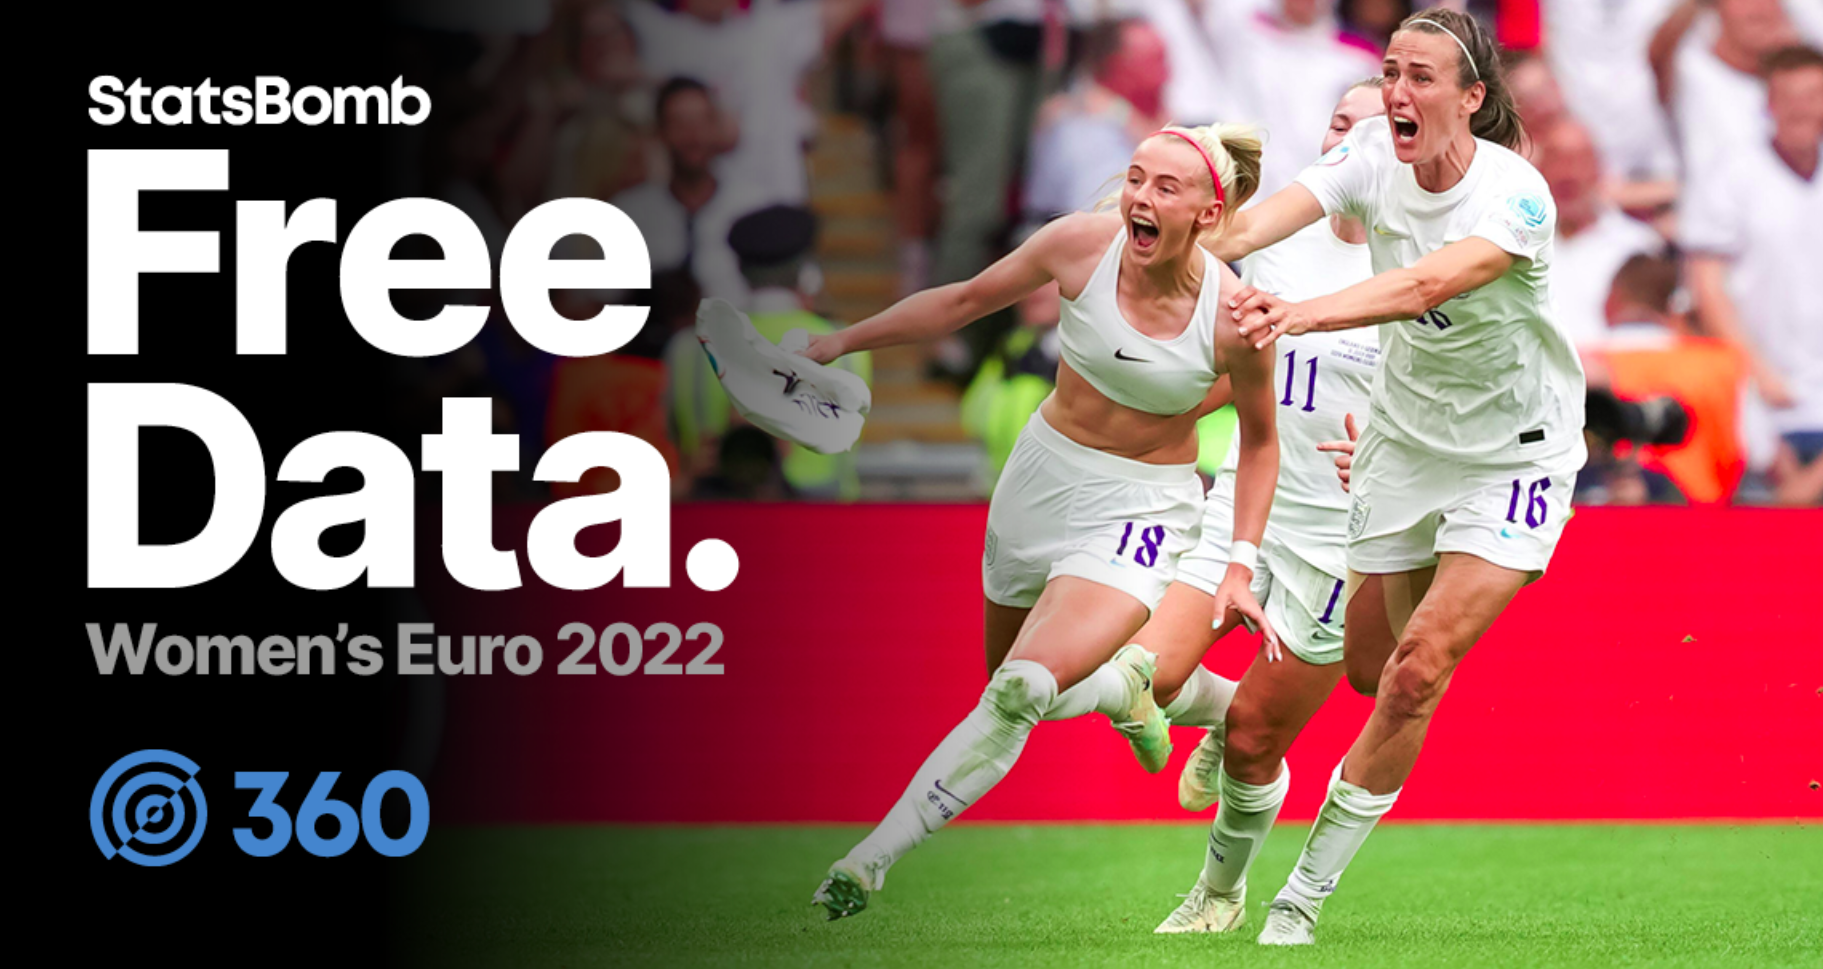
\includegraphics[width=0.35\textwidth,keepaspectratio]{free_data.png}
		\\
		\footnotesize(Nunca antes se habían liberado datos 360 de StatsBomb para fútbol femenino)
    \end{center}
\end{frame}

\begin{frame}{Preprocesamiento de datos}
	\begin{itemize}
		\item FreeCompetitions
		\item FreeMatches
		\item Guardamos los de Inglaterra y Noruega y les extraemos los eventos
		\item 2246 pases completos de Inglaterra a lo largo de la EURO 2022 vs 967 de Noruega.
		\item 444 pasess completos de Inglaterra en el partido Inglaterra-Noruega vs 177 de Noruega.
	\end{itemize}
	\begin{columns}[t]
		\column{.5\textwidth}
		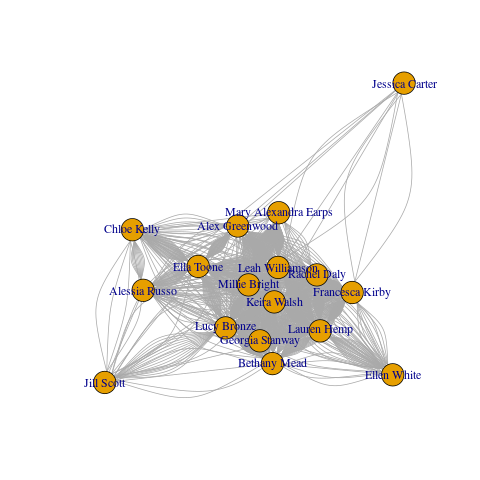
\includegraphics[width=\columnwidth,height=3cm]{plot_england.png}
		\footnotesize(Red de pases total de Inglaterra)
		\column{.5\textwidth}
		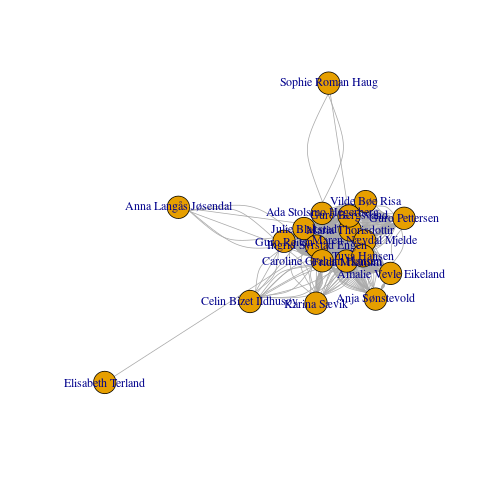
\includegraphics[width=\columnwidth,height=3cm]{plot_norw.png}
		\footnotesize(Red de pases total de Noruega)
	\end{columns} 
\end{frame}

\begin{frame}{Redes de pases a lo largo de la competición}
    \begin{columns}[t]
        \column{.5\textwidth}
        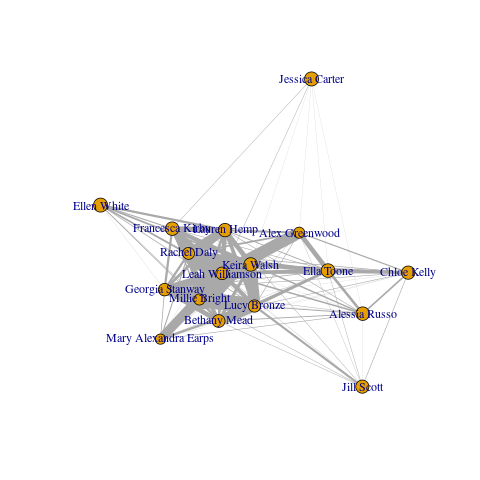
\includegraphics[width=\columnwidth,height=3cm]{plot_england_simpl.png}
        \footnotesize(Red de pases total simplificada de Inglaterra)
        \column{.5\textwidth}
        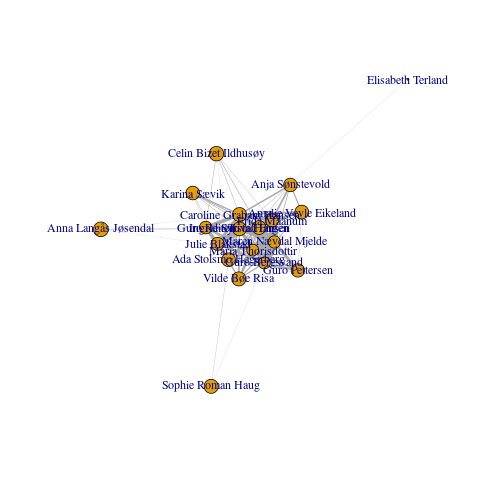
\includegraphics[width=\columnwidth,height=3cm]{plot_norw_simpl.png}
        \footnotesize(Red de pases total simplificada de Noruega)
    \end{columns} 
	\begin{alertblock}{Nota}
		\textlatin{La entropía por jugadora es el tamaño de cada nodo. El grosor de los enlaces es el 
	 	número de pases que ha habido.}
	\end{alertblock}
\end{frame}

\begin{frame}{Partido Inglaterra 8 - Noruega 0}
		\begin{columns}[t]
			\column{.5\textwidth}
			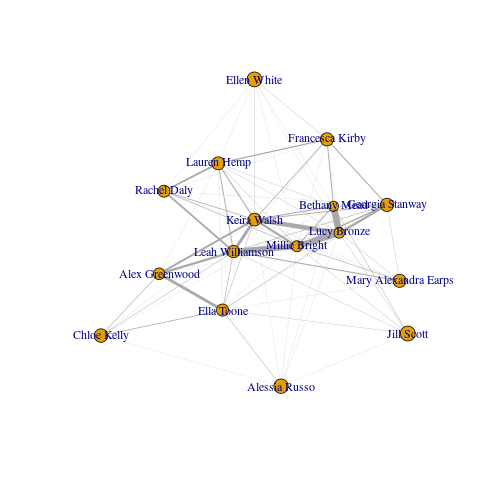
\includegraphics[width=\columnwidth,height=3cm]{entropy_match_engl_simpl.png}
			\captionof{figure}{Red de pases simplificada de Inglaterra}
			\column{.5\textwidth}
			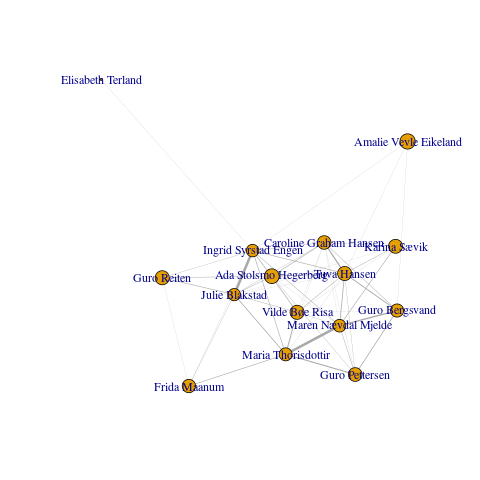
\includegraphics[width=\columnwidth,height=3cm]{entropy_match_norw_simpl.png}
			\captionof{figure}{Red de pases simplificada de Noruega}
		\end{columns} 
\end{frame}

\begin{frame}{Comparativa por jugadoras a lo largo de la competición}
	\begin{figure}
		\centering
			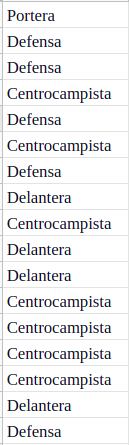
\includegraphics[width=0.105\textwidth]{positions_england_total.png}
			\subfloat[Entropía total de Inglaterra]{
			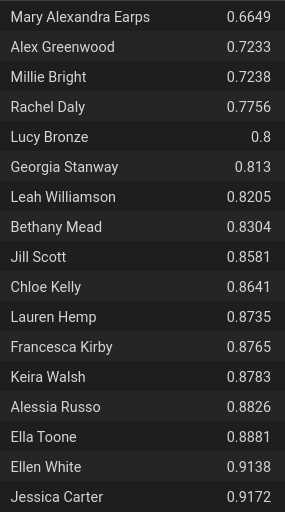
\includegraphics[width=0.2\textwidth]{england_total_ordered.png}}
			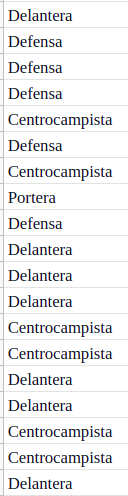
\includegraphics[width=0.101\textwidth]{positions_norway_total.png}
			\subfloat[Entropía total de Noruega]{
			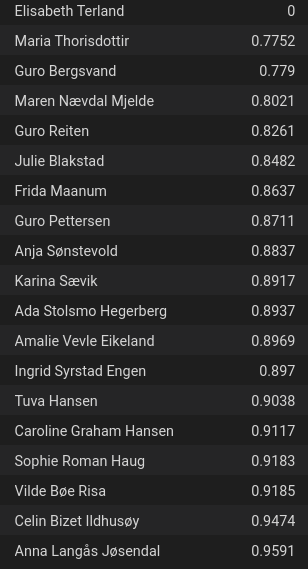
\includegraphics[width=0.21\textwidth]{norway_total_ordered.png}}
		\end{figure}
\end{frame}

\begin{frame}{En el partido Inglaterra 8-Noruega 0}
	\begin{figure}
		\centering
			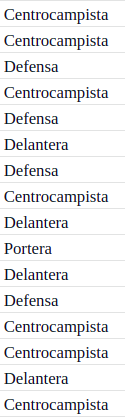
\includegraphics[width=0.101\textwidth]{positions_england_match.png}
			\subfloat[Entropía total de Inglaterra]{
			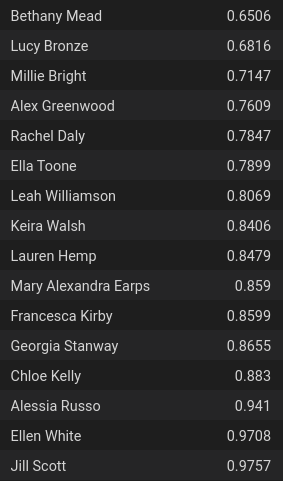
\includegraphics[width=0.199\textwidth]{england_match_ordered.png}}
			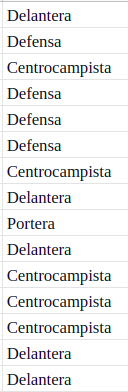
\includegraphics[width=0.102\textwidth]{positions_norway_match.png}
			\subfloat[Entropía total de Noruega]{
			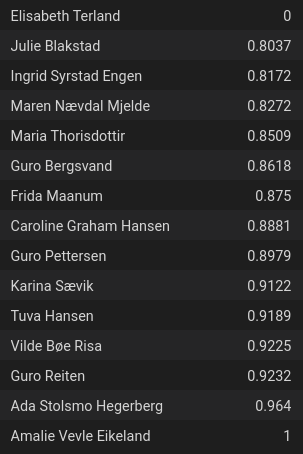
\includegraphics[width=0.209\textwidth]{norway_match_ordered.png}}
		\end{figure}
\end{frame}

\begin{frame}{Interpretaciones}
	\begin{columns}[t]
		\column{.5\textwidth}
		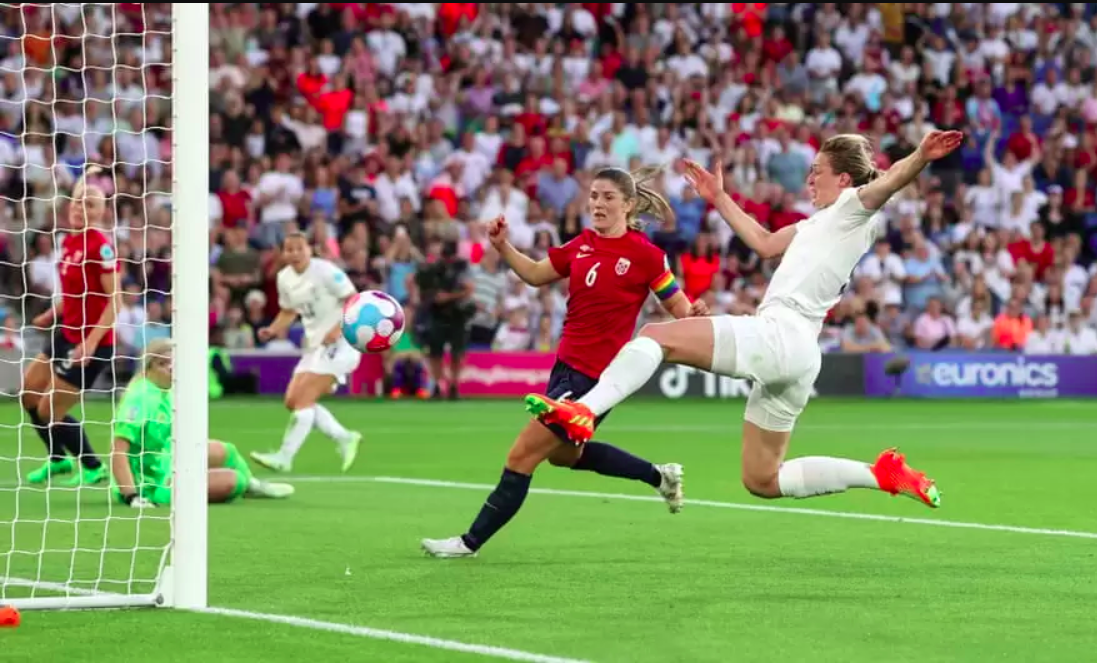
\includegraphics[width=\columnwidth,height=3cm]{white.png}
		\footnotesize(White- 0.9708, Mjelde (6)- 0.8272)
		\column{.5\textwidth}
		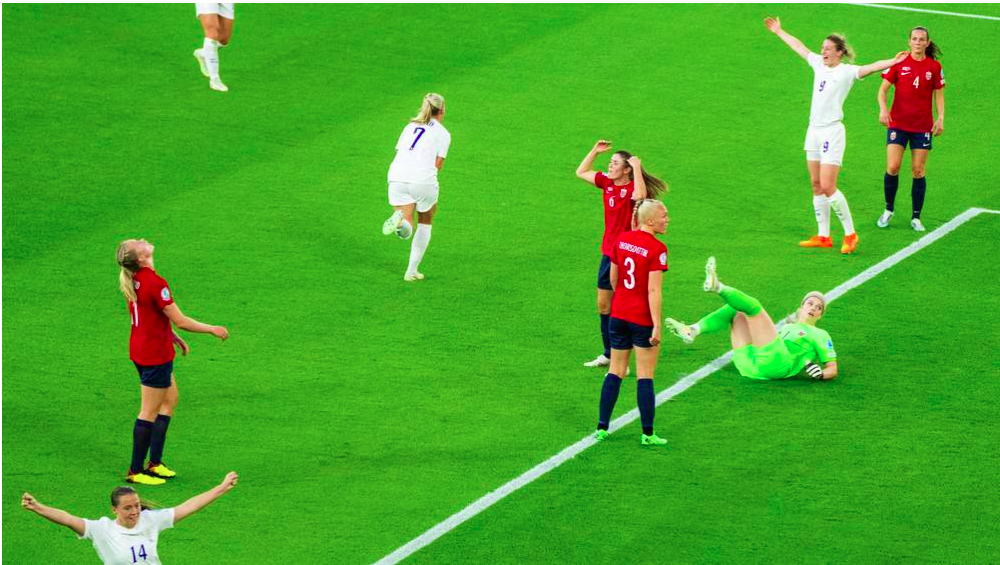
\includegraphics[width=\columnwidth,height=3cm]{norw2.png}
		\footnotesize(Mead (7)- 0.6506, White (9), Kirby (14)- 0.8599, Thorisdottir(3)- 0.8509, Tuva Hansen(4)- 0.9189)
	\end{columns} 
\end{frame}

\begin{frame}{Resultados}
	\begin{alertblock}{Principio de máxima entropía de Jayne}
		Entre todas las distribuciones, debemos elegir aquella con la entropía máxima, esto es, 
		la que tiene mayor variabilidad.
	\end{alertblock}
	\begin{figure}
		\centering
			\subfloat[Entropía total de Inglaterra]{
			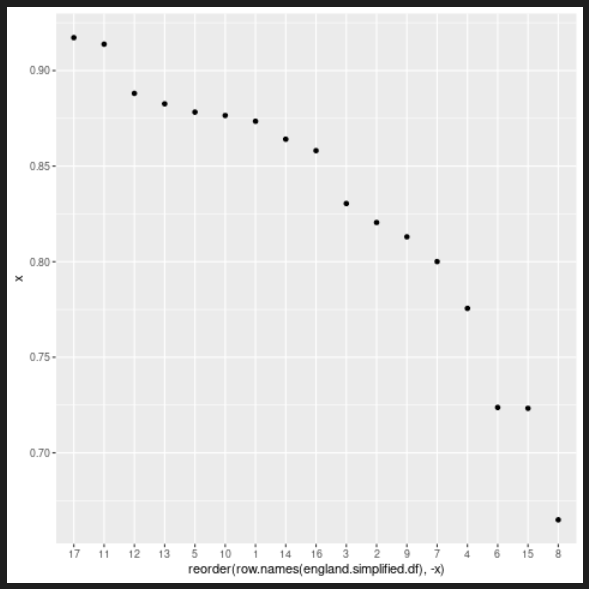
\includegraphics[width=0.4\textwidth]{englandentropy.png}}
			\subfloat[Entropía total de Noruega]{
			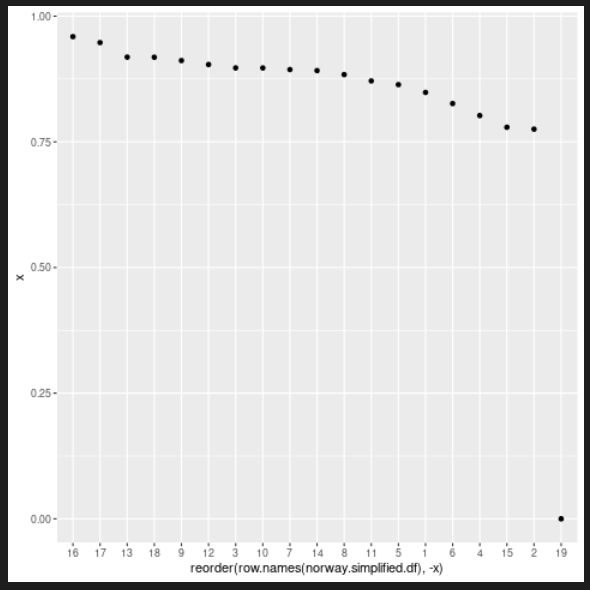
\includegraphics[width=0.4\textwidth]{norwayentrop.png}}
	\end{figure}
\end{frame}

%
\subsection{Conclusiones y trabajos futuros}

\begin{frame}{Conclusiones}
	\begin{itemize}
		\item Con la entropía sobre el grafo de pases podemos explicar el desempeño de un equipo
		\item Entropía a nivel de jugador y de equipo
		\item Se puede ver la ``mejor'' o ``peor'' entropía reflejada en un tipo de 
		visualización de las redes de pases
	\end{itemize}
\end{frame}

\begin{frame}{Trabajos futuros}
	Profundización en redes bayesianas para:
	\begin{itemize}
		\item Influencia del rival
		\item Posesión del balón
		\item Minutos jugados de cada jugadora
		\item Entropía espacio-temporal
		\item Alineación y cambios
	\end{itemize}
\end{frame}

\section{Extra}

\begin{frame}{Preguntas}
	\begin{center}
		Det er alt, folkens! \\[12pt]
		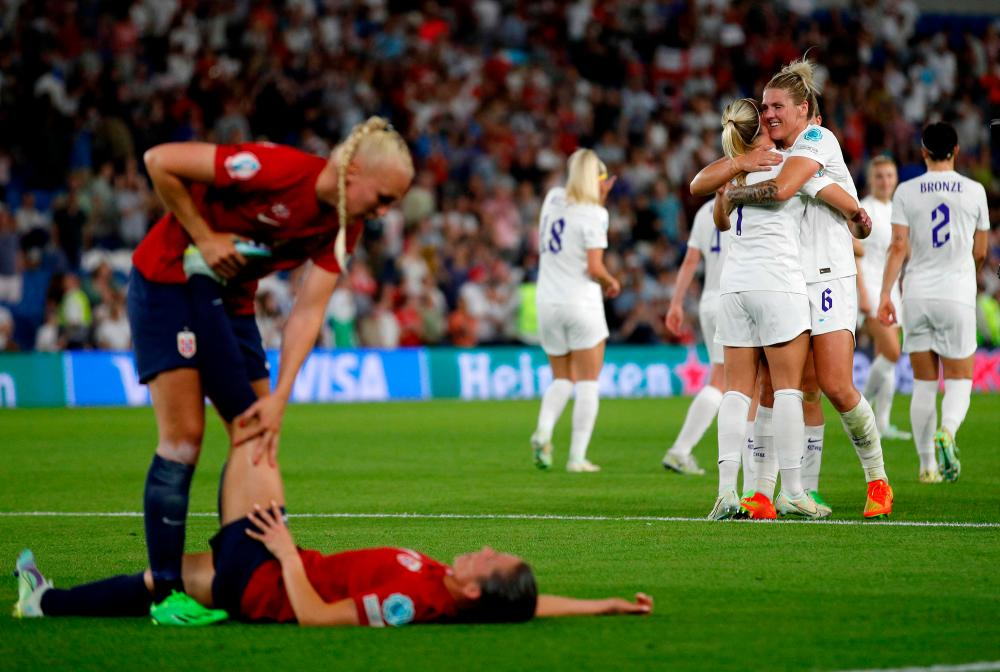
\includegraphics[width=0.75\textwidth,keepaspectratio]{final.jpg}
    \end{center}
\end{frame}

\begin{frame}{Asignaturas usadas}
	\begin{itemize}
		\item Estadística descriptiva e introducción a la probabilidad 
		\item Inferencia estadística 
		\item Probabilidad 
		\item Estadística computacional 
		\item Infraestructura Virtual
	\end{itemize}
\end{frame}

\begin{frame}{Costes}
	\begin{table}
		\begin{tabular}[h!tbp]{lccr}
		  Concepto & Coste unitario & Unidades & Total \\
		  Amortización portátil & 150€ & 1 & 150€ \\
		  Ventilador            & 14€  & 1 & 14€ \\
		  Costes laborales      & 2000€& 3.5 & 7000€ \\
		  \hline \\
		  \multicolumn{3}{l}{Total} & 7164€ \\
		\end{tabular}
		\caption{Costes el proyecto en el escenario ``analista de datos junior''} \label{tab:costes2}
		\end{table}
\end{frame}

\begin{frame}{Redes bayesianas}
	\begin{center}
		Ejemplo de grafo dirigido acíclico \\[12pt]
		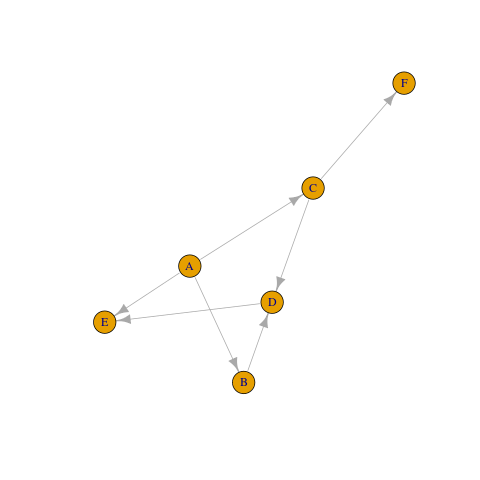
\includegraphics[width=0.35\textwidth,keepaspectratio]{dag.png}
		\\
		\footnotesize(Una red bayesiana consiste en un modelo estructural y un conjunto de probabilidades)
    \end{center}
\end{frame}

\begin{frame}{Entropía + Redes bayesianas}
	\begin{itemize}
		\item Para calcular la entropía de Shannon debe cumplirse la propiedad de aditividad 
		\item $P(A U B) = P(A) + P(B) - P(A \cap B)$; para que sea aditiva la probabilidad de la intersección 
		debe ser 0, pero $P(A \cap B) = P(A)P(B/A)$
	\end{itemize}
	\begin{alertblock}{Entropía de Tsallis}
		Para modelar el sistema con redes bayesianas, habría que usar una entropía que sí 
		cumpliera esas propiedades.
		La entropía de Shannon, implementada en igraph, refleja la propiedad (caos/orden/sorpresa) que 
		estamos buscando, lo que fue suficiente para la viabilidad del producto en esta fase.
	\end{alertblock}
	
\end{frame}

\begin{frame}{Redes causales}
   \begin{block}
        <1->{}
            \begin{itemize}
                \item Red bayesiana en la que los padres de cada nodo son sus causas directas.
                \item Satisface la {\em condición de Markov causal}
            \end{itemize}
    \end{block}
    \begin{exampleblock}
        <2->{Condición de Markov causal}
            \begin{itemize}
                \item Dadas las causas directas, el fenómeno asociado a un nodo es independiente de 
                los que no tienen efecto sobre él. Esta asunción permite que la distribución 
                conjunta de las variables en una red causal sea factorizada como :
                $$ P(X_{1}, \dots,X_{N}) = \prod_{i=1}^{N} P(X_{i} | pa(X_{i}))$$ 
            \end{itemize}
    \end{exampleblock}
\end{frame}

\begin{frame}{Entropía de Tsallis}
Con la entropía de Tsallis de los pases entre los jugadores, se puede medir la organización asociada al 
comportamiento de un equipo de fútbol. Fue diseñada para analizar sistemas donde existen correlaciones 
entre sus microestados
	\begin{definition}[Entropía de Tsallis] 
	Dado un conjunto discreto de probabilidades ${p_i}$ con la condición $\sum_{i} p_i = 1$, y con $q$ 
	cualquier número real, se define la entropía de Tsallis como
	$$ S_q(p_i)=\frac{k}{q-1}\left(1- \sum_{i=1}^{N}p_{i}^{q}\right)$$
	donde $q$ se denomina índice entrópico, $N$ son los microestados y $k$ es una constante positiva.
	\end{definition}
La fórmula se reduce a la de la entropía de Shannon cuando $q=1$.
\end{frame}

%%
\end{document}